\chapter{Overview of previous work in the field of crop row detection}
\label{sec:latexumg}

A lot of research has been done to autonomously detect crop rows using computer vision.The main approaches are LiDAR based techniques, CNN's, and more classical Machine Vision approaches. \\

\section{LiDAR based techniques}


As \citet{AgricultureLiDARZhang} and \citet{LiDARCHangingplantgrowth} have shown,  height information can be used to detect crop rows. However, while the detection of crops during the late period is successful with LiDAR, this technique is not reliable when it comes to the detection of tiny plants, in the early stages of development. The cost of LiDAR sensors is also high and is not suitable for large-scale configuration of agricultural vehicles.   

\section{Convolutional Neural Networks}
CNN can also be used to process images of crop rows and detect rows in new images (\citet{CNN1}, \citet{thesisDOHA}, \citet{DeepLearning2}). However, deep learning methods are limited by the available datasets. As the appearance of the crop row varies a lot depending on the type of crop, the growth stage, the environmental condition and the weather condition, the required dataset must be huge. In our case, we would also need images taken from the same height and angle as our rover.  Today, such large-scaled datasets are not available, and acquiring our own would be very difficult, time consuming, and should be done at various seasons of the year and on various crops.

\section{Classical Machine Vision approach}


\subsection{Segmentation}

To distinguish crops from the background, segmentation is usually performed using color index-based segmentation followed by threshold-based segmentation (\cite{VEGEIDX}). 

Color index segmentation is widely used in agricultural image processing, the most common being the Excess Green Index (ExG, \cite{ExgreenIdx}), the Color Index of Vegetative Extraction (CIVE, \cite{CIVE}) and the normalized difference vegetation index (NDVI, \cite{NDVI}). Post-processed, the new gray image has higher-intensity pixels where the vegetation is. 

Once the image is grayscaled, it is usually binarized. The selection of the threshold has to be very well tuned. 
A common technique is to use Otsu thresholding (\citet{4310076}), which autonomously finds a threshold that maximizes the variance between the foreground (the vegetation) and the background. This works by iterating through all possible threshold values and for each one, calculating the variance (how much the intensities in each group differ from the group's mean intensity) between the two groups of pixels. \\

As these techniques are highly sensitive to light changes, some use learning-based segmentation, mainly deep learning, to obtain the best segmentation values (\citet{deepLforSeg}). 

Since no large dataset for vegetation segmentation was accessible, here a threshold-independent segmentation method using color clustering was developed, which will be described later.

\subsection{Line-detection}

Once the vegetation is segmented and a binary image has been computed, a line detection algorithm is necessary to extract crop rows. Currently, the most commonly used line-fitting techniques are the Hough transform, the least squares method, and the Random Sample Consensus. 

\subsubsection{Hough Transform}
\label{subsubsection:HT}

Used to detect lines, circles, or more complex shapes, the Hough transform converts the pixel space to a parameter space, as illustrated in Fig. \ref{fig:HOUGHTRANS}
In the case of line detection, each line in the image is described by the parameters $\rho$  and $\theta$ as such : 
\begin{equation}
\rho(\theta) = x_{0} \cdot \cos{\theta} + y_{0} \cdot \sin{\theta} 
\end{equation}




The Hough space is defined as a graph with abscissa $\theta$ and $\rho$, so each point ($\theta_{i}$, $\rho_{i}$) describes a line in the image space. Once each pixel of an image is mapped to the Hough space, the intensity values at a certain point ($\theta_{i}$, $\rho_{i}$) will be higher when this point describes a prominent line in the image pixels plane. 

This technique is one of the most widely used (\citet{HTRTTracking}) but, on its own, it is not sufficient to detect crop rows robustly. It is highly sensitive to noise (lightning, shading, bushiness, various stages of growth), which requires substantial manual tuning and can lead to false detection of lines. In a region of high weed pressure, many lines are feasible. It is also computationally expensive and difficult to use for real-time applications. 

\begin{figure}[H]
\begin{minipage}{0.5\columnwidth}
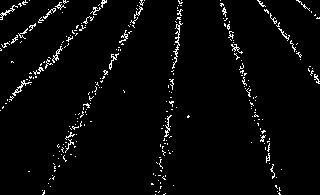
\includegraphics[width=\columnwidth,height=4cm]{Report/images/ImageProcesses/HoughProcess/VegeMask.png}
\\[3mm]
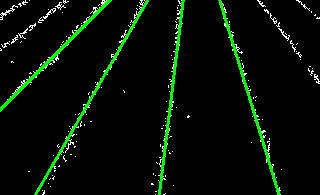
\includegraphics[width=\columnwidth,height=4cm]{Report/images/ImageProcesses/HoughProcess/HoughLineDrawned.png}
\captionsetup{justification=centering}
\subcaption{Line detected in Image Space by the Hough Process}
\end{minipage}
\hspace{1cm}
\begin{minipage}{0.8\columnwidth}
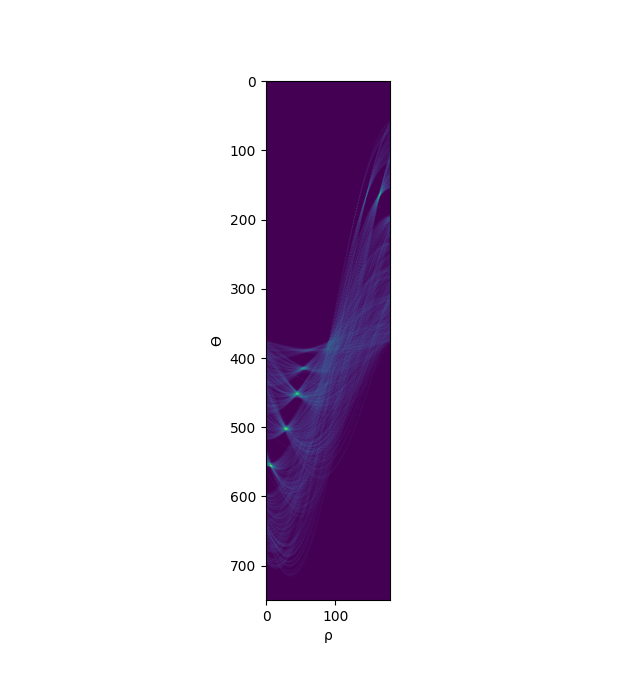
\includegraphics[width=\columnwidth,height=83mm]{Report/images/ImageProcesses/HoughProcess/HoughAcc.png}
\captionsetup{justification=centering}
\subcaption{ Accumulator in the Hough Space\\ $\rho$ [pixel count], $\theta$ [rad]}

\end{minipage}
\hspace{1cm}
\caption{Illustration Hough process}        
\label{fig:HOUGHTRANS}

\end{figure}


\subsubsection{Least square}

\citet{LeastSquares2} and \citet{LeastSquares} use least squares to fit the different rows of crops. Although faster and more robust to weeds, this technique requires prior knowledge to fit the template, such as the number of crop rows to be detected, the expected location of each crop row, and the area to be explored in the image. \\


\subsubsection{RANSAC}

RANSAC (RANdom SAmple Consensus) is an iterative algorithm for estimating the parameters of a mathematical model from a set of observed data that contains outliers (i.e. data that do not fit the model). Here, it is used for line fitting, and the model is defined by the slope and a point on the line. The basic idea behind it is to randomly select a subset of the data points (2 inliers are selected for line fitting) and use them to estimate the parameters of the model. The remaining points (the outliers) are then used to test the validity of the model. This process is repeated multiple times, and the model with the most inliers is chosen as the final solution. The inliers are the points that fall within a certain distance threshold from the line, and the outliers are the points that fall outside of this threshold. RANSAC is a robust algorithm that can handle outliers and still find the correct solution - in our case, it will eliminate weeds or vegetation in between crops. It is faster than the complete Hough transform method and, thus, more adapted for real-time applications.


However, as with the least squares method, some prior information on crop rows is necessary: \citet{RANSACbase} based their RANSAC process on a skeleton of the row features. \\ \\ \\ \\

\begin{figure}[H]
\centering
\begin{subfigure}{0.49\textwidth}
    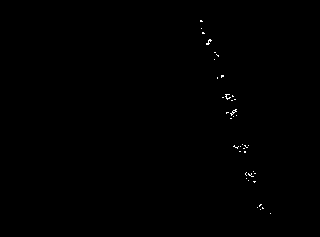
\includegraphics[width=\textwidth]{Report/images/masked images _ransac.png}
    \label{fig:singlelinemask}
\end{subfigure}
\begin{subfigure}{0.49\textwidth}%
    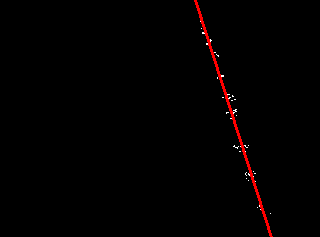
\includegraphics[width=\textwidth]{Report/images/masked images _ransacfitted.png}
    \label{fig:ransacfitsingline}
\end{subfigure}

\caption{Results of the RANSAC algorithm for line fitting}
\end{figure}
\label{pics: Ransacmasking}

\vspace{20mm}

In this project, an algorithm is developed that combines different methods to make each of them more robust and efficient. Hough transform is used as a preprocessing step to calculate the vanishing point and the approximate location of crops, the vanishing point is used to detect outlier lines not parallel in world coordinates, and RANSAC is used to detect the center of each crop rows. 







